\section{Methods: sector matrices, closures and certificates}\label{sec:methods}

This section gives the three algorithms behind Section~\ref{sec:results6}: the computation of the six sector matrices
of a block (Algorithm~\ref{alg:sector}), the closure of a family of blocks kept as an antichain under containment
(Algorithm~\ref{alg:closure}), and the independent check of the resulting certificate (Algorithm~\ref{alg:check}).
Their parameters are those of the computations EXP-013 and EXP-014 (library module \texttt{code/pcclib/transfer.py},
runner \texttt{run.py}, checker \texttt{check\_certificate.py}).

\subsection{Encoding of a block}\label{sec:encoding}

The formula of a 6-pole with $n$ vertices has $q = (3n + 6)/2$ items: $(3n - 6)/2$ internal edges, since the six
dangling ends account for six of the $3n$ edge ends, plus the six ends. By Equation~\eqref{eq:size-pole} without the two
unit clauses of fixed labels, it has
\begin{equation}\label{eq:size-block}
15\,q \text{ variables and } 106\,q + 495\,n \text{ clauses.}
\end{equation}
The claw ($n = 4$, $q = 9$) has \nVarsBlockY{} variables and \nClausesBlockY{} clauses; the superedge ($n = 8$, $q = 15$) has
\nVarsBlockS{} and \nClausesBlockS{}; a 6-pole of $\PG$ of shape~(b) ($n = 10$, $q = 18$) has \nVarsBlockPb{} and
\nClausesBlockPb{}; a 6-pole of $J_5$ or of the dodecahedron of shape~(a) ($n = 18$, $q = 30$) has \nVarsBlockJa{} and
\nClausesBlockJa{}; one of $J_7$ ($n = 26$, $q = 42$) has \nVarsBlockJs{} and \nClausesBlockJs{}. The formulas are small; what
makes the largest blocks slow is the number of solver calls of Algorithm~\ref{alg:sector}, not the size of the formula.
The labels of the left connector are not fixed by unit clauses: Algorithm~\ref{alg:sector} passes them as assumptions, so that one formula serves all
left triples of a block and the clauses learned for one triple help the next. For the class $\Oz$ the sector has $60 = 10 \cdot 6$ ordered triples, the ten stars of $\PG$ in the six
orders of their three edges, since a class-$\Oz$ triple with a repeated label is impossible. The other sector orders, $67, 48, 48, 30, 60$, count the ordered triples of labels, repetitions
allowed, whose class equals the representative class of the orbit, and the six orders add up to $15^3$ over the 64 classes (Equation~\eqref{eq:sectors}).

\subsection{Sector matrices of a block}\label{sec:alg-sector}

\begin{algorithm}[t]
\caption{Sector matrices of a block (projected model enumeration).}\label{alg:sector}
\DontPrintSemicolon
\KwIn{a block $M$ with ordered connectors $L = (l_1, l_2, l_3)$, $R = (r_1, r_2, r_3)$; the six sets $S_o$ of ordered label triples of the representative class of each orbit $o$}
\KwOut{six boolean matrices $T^o$ of orders $n_o = |S_o|$, equal to the restriction of $T_M$ to $S_o \times S_o$}
build the formula $F_M$ of Section~\ref{sec:encoding}; open one incremental CaDiCaL solver on $F_M$\;
\For{each orbit $o$ and each triple $a \in S_o$}{
  take a fresh selector literal $\mathit{sel}$\;
  \While{the solver finds a model under the assumptions $y_{l_k, a_k}$ ($k = 1,2,3$) and $\mathit{sel}$}{
    read $b = (\text{labels of } r_1, r_2, r_3)$ from the model\;
    \lIf{the model fails the star-condition checker, or $b \notin S_o$, or the labels of $L$ differ from $a$}{abort}
    set $T^o[a, b] \leftarrow 1$\;
    add the clause $\neg\mathit{sel} \lor \bigvee_k \neg y_{r_k, b_k}$ \Comment*[r]{block this right triple}
  }
  add the unit clause $\neg\mathit{sel}$ \Comment*[r]{retire the selector}
}
\Return{$T^o$ for the six orbits}
\end{algorithm}

Algorithm~\ref{alg:sector} enumerates, for each of the $\sum_o n_o = \nTripleSum$ left triples $a$ of the six
representative classes, all right triples $b$ that extend to a map with every vertex good. Entries are models read back
and checked from the definition, never inferred; the unrestricted block has $15^3$ left triples but conduction
(Proposition~\ref{prop:sectors}) reduces the work to the six representative classes. One solver serves all calls of a block, so
learned clauses are reused. The number of solver calls of a block is
\begin{equation}\label{eq:calls}
N_{\mathrm{calls}}(M) \;=\; \sum_o n_o \;+\; \sum_o \bigl|T^o\bigr| ,
\end{equation}
one call per model and one unsatisfiable call per left triple. The claw has \nCallsClaw{} calls and the superedge
\nCallsSuperedge{}, with $\nSuperedgeZero$, $\nSuperedgeE$ and $\nSuperedgeDtwo$ entries in the sectors $\Oz$, $\OEc$ and
$\ODtwo$ of the superedge and none in the others. The 81 blocks of Table~\ref{tab:blocks} took \nBlockTotal{} seconds of solver time in
all (mean $\nBlockMean \pm \nBlockSd$ seconds per block, sample standard deviation), the slowest one \nBlockSlowest{} seconds
(Figure~\ref{fig:blocktimes}).

\begin{figure}[t]\centering
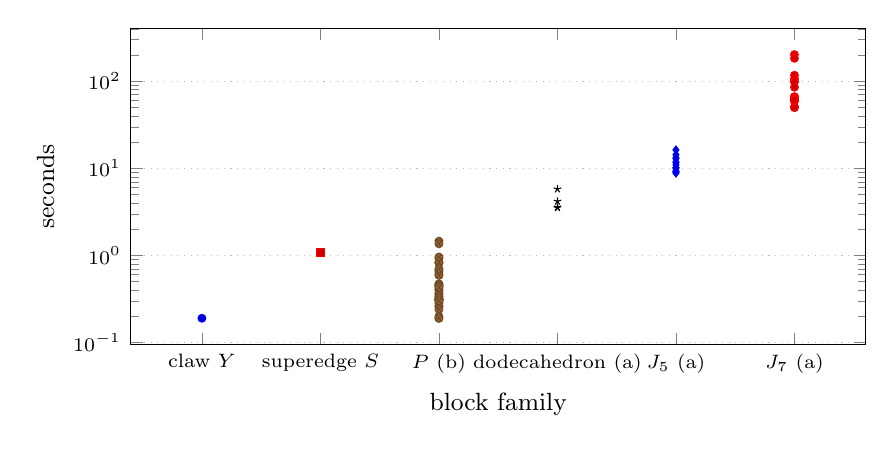
\begin{tikzpicture}
\begin{axis}[width=0.9\textwidth,height=5.6cm,ymode=log,only marks,mark size=1.4pt,symbolic x coords={Y,S,Pb,Da,Ja5,Ja7},xtick={Y,S,Pb,Da,Ja5,Ja7},xticklabels={claw $Y$,superedge $S$,$P$ (b),dodecahedron (a),$J_5$ (a),$J_7$ (a)},x tick label style={font=\scriptsize},ylabel={seconds},xlabel={block family},tick label style={font=\scriptsize},label style={font=\small},enlarge x limits=0.12,ymajorgrids=true,grid style={dotted}]
\addplot coordinates {(Y,0.19)};
\addplot coordinates {(S,1.09)};
\addplot coordinates {(Pb,1.46) (Pb,0.82) (Pb,1.36) (Pb,0.31) (Pb,0.83) (Pb,0.65) (Pb,0.93) (Pb,0.83) (Pb,0.96) (Pb,0.61) (Pb,0.69) (Pb,0.36) (Pb,0.4) (Pb,0.41) (Pb,0.32) (Pb,0.31) (Pb,0.3) (Pb,0.28) (Pb,0.59) (Pb,0.46) (Pb,0.26) (Pb,0.26) (Pb,0.47) (Pb,0.31) (Pb,0.47) (Pb,0.32) (Pb,0.37) (Pb,0.34) (Pb,0.24) (Pb,0.31) (Pb,0.45) (Pb,0.34) (Pb,0.44) (Pb,0.32) (Pb,0.43) (Pb,0.19) (Pb,0.2) (Pb,0.7) (Pb,0.19) (Pb,0.3)};
\addplot coordinates {(Da,5.78) (Da,4.18) (Da,3.58) (Da,3.52)};
\addplot coordinates {(Ja5,11.76) (Ja5,10.16) (Ja5,11.78) (Ja5,8.91) (Ja5,8.84) (Ja5,9.34) (Ja5,14.37) (Ja5,12.89) (Ja5,10.18) (Ja5,10.99) (Ja5,16.27) (Ja5,13.27) (Ja5,9.2) (Ja5,10.05)};
\addplot coordinates {(Ja7,117.18) (Ja7,99.73) (Ja7,106.37) (Ja7,62.1) (Ja7,63.44) (Ja7,66.49) (Ja7,66.09) (Ja7,62.57) (Ja7,65.53) (Ja7,202.28) (Ja7,98.12) (Ja7,63.69) (Ja7,63.43) (Ja7,62.66) (Ja7,58.72) (Ja7,183.29) (Ja7,85.4) (Ja7,61.0) (Ja7,61.46) (Ja7,50.95) (Ja7,49.72)};
\end{axis}
\end{tikzpicture}

\caption{Computation time of the six sector matrices of each of the 81 blocks, by block family (computation EXP-014, \texttt{blocks.json}); the time grows with the
number of vertices of the block and with the number of entries, and the slowest block, in the $J_7$ family, took 202 seconds.}\label{fig:blocktimes}
\end{figure}

\subsection{Independent recomputation of the matrices}\label{sec:alg-recheck}

Two independent computations test the completeness of Algorithm~\ref{alg:sector}. The first is a brute-force
enumeration with no solver: a backtracking search over the vertices of the block that chooses for each vertex a star of $\PG$ and one of the
six bijections of its three items onto the three edges of the star, rejects choices that disagree with labels already
assigned, and collects the pairs (labels of $L$, labels of $R$). It is feasible for the claw and the superedge. The second
is a different encoding, with one Boolean variable per vertex, image vertex of $\PG$ and bijection (at least one per vertex,
each choice implying the labels of its three items), pairwise exactly-one constraints on labels, and a different
solver, MiniSat 2.2, enumerating the same projected models. The matrices of the two computations are compared entrywise: equality means that the six boolean matrices coincide
in every entry, so neither computation finds an entry that the other misses. The brute-force enumeration depends on no propositional encoding at all.
The second encoding shares with the first only the definition of the sector states and the extraction of the right triple, and its solver is a different implementation
(MiniSat 2.2 against the CaDiCaL 1.5.3 interface of PySAT). The run that recomputed the blocks by the second encoding was stopped by a limit of ninety minutes, which is why
46 of the 81 blocks were reached.

\subsection{Closure of a block family}\label{sec:alg-closure}

A family $\mathcal{F}$ yields its generators $\mathcal{G}$ as in Corollary~\ref{cor:semigroup}: for every block, both orientations and the
six junction permutations, with equal six-tuples identified. The exact closure is the set of all products of at least
two generators, computed breadth first by right multiplication, deduplicated on the packed bytes of the six matrices.
The \emph{antichain} closure of Algorithm~\ref{alg:closure} keeps only the elements minimal under entrywise containment;
it is the method used for the certificates, because a product that contains a kept element contains a certificate element
and needs no further expansion (Corollary~\ref{cor:semigroup}).

\begin{algorithm}[t]
\caption{Antichain closure of a family of generators with a certificate.}\label{alg:closure}
\DontPrintSemicolon
\KwIn{generators $g_1, \dots, g_k$ (six-tuples of boolean matrices); a cap $N$ on the stored elements (200{,}000); a time limit $\tau$ imposed on the process}
\KwOut{a certificate $\mathcal{C}$ and the list of zero-trace elements, or \textsf{undecided}}
$\mathcal{C} \leftarrow \emptyset$; queue $Q \leftarrow \emptyset$\;
\For{$i, j \in \{1, \dots, k\}$}{ \textsf{offer}$(g_i g_j)$ }
\While{$Q \ne \emptyset$}{
  \lIf{more than $N$ elements are stored, or the time exceeds $\tau$}{\Return{\textsf{undecided}}}
  remove $x$ from $Q$; \lIf{$x$ was retired}{continue}
  \For{$j \in \{1, \dots, k\}$}{ \textsf{offer}$(x\, g_j)$ }
}
\Return{$\mathcal{C}$ and every stored element whose diagonal is zero in all six sectors}\;
\BlankLine
\textbf{procedure} \textsf{offer}$(x)$\;
\Indp
\lIf{some $c \in \mathcal{C}$ is contained in $x$ entrywise, or $x$ is already stored}{drop $x$}
\Else{
  retire and remove from $\mathcal{C}$ every $c' \in \mathcal{C}$ that contains $x$ \Comment*[r]{retired elements are not expanded}
  add $x$ to $\mathcal{C}$ and to $Q$; record its first parent, so that its word in the generators can be read back\;
}
\end{algorithm}

Candidates produced from one expanded element are offered in increasing number of nonzero entries, so that smaller elements
retire larger ones before the larger ones are stored. At termination every product of at least two generators contains an
element of $\mathcal{C}$ and every element of $\mathcal{C}$ times every generator does too, which are the conditions of
Corollary~\ref{cor:semigroup}; the nonzero diagonal of each element is tested at the moment the element is stored.

The cost is governed by three numbers. Each expansion multiplies the current element by the $k$ generators, each product
costing $\sum_o n_o^3 = \nCubeSum$ boolean multiply-adds, done as single-precision floating-point matrix products on the six sectors at once. The exact closure
therefore costs about $|\Sigma|\cdot k \cdot \sum_o n_o^3$ operations,
\begin{equation}\label{eq:cost}
\mathrm{cost}_{\mathrm{exact}} \;\approx\; |\Sigma| \cdot k \cdot \sum_o n_o^3 \;=\; 116{,}463 \cdot 12 \cdot 980{,}947 \;\approx\; 1.4\times 10^{12}
\end{equation}
for the family $F_3 = \{Y, S\}$, and $19{,}005\cdot 6\cdot 980{,}947 \approx 1.1\times 10^{11}$ for $F_2 = \{S\}$. The antichain
closure expands only the elements that stay minimal and adds a containment test of each candidate against the kept elements,
which are stored as $17{,}197$ bits, padded to 269 machine words of 64 bits (2{,}152 bytes), so that one test costs at most $269$ word
operations per kept element. The array of kept elements has $N + 1 = 200{,}001$ rows, about 430 megabytes. The cap $N = 200{,}000$ and the time limits are
parameters, not properties of the method: an exact closure that reaches the cap, or an antichain closure that is stopped at its one-hour
limit, is reported as undecided and proves nothing about the family.

\subsection{Check of a certificate}\label{sec:alg-check}

\begin{algorithm}[t]
\caption{Certificate check with integer products.}\label{alg:check}
\DontPrintSemicolon
\KwIn{the stored block matrices; the stored generators and certificate $\mathcal{C}$ of a family; its blocks and junction permutations}
\KwOut{\textsf{accept} or \textsf{reject}}
rebuild the generators $g_1, \dots, g_k$ from the stored block matrices; \lIf{they differ from the stored generators}{\Return{\textsf{reject}}}\;
\For{$i, j \in \{1, \dots, k\}$}{ compute $p = g_i g_j$ with 32-bit integer matrix products and threshold at $0$\; \lIf{no $c \in \mathcal{C}$ is contained in $p$ entrywise}{\Return{\textsf{reject}}} }
\For{$c \in \mathcal{C}$ and $j \in \{1, \dots, k\}$}{ compute $p = c\, g_j$ by integer products\; \lIf{no $c' \in \mathcal{C}$ is contained in $p$ entrywise}{\Return{\textsf{reject}}} }
\lIf{some $c \in \mathcal{C}$ has a zero diagonal in all six sectors}{\Return{\textsf{reject}}}
\Return{\textsf{accept}}
\end{algorithm}

Algorithm~\ref{alg:check} shares no code with the closure runner except the storage format. It recomputes the boolean
products by integer matrix multiplication followed by a threshold, where the runner uses single-precision floating point,
and it tests containment of every product in the certificate instead of trusting the runner's bookkeeping. It performs $k^2 + |\mathcal{C}|\,k$ products;
for $F_3$ this is $12^2 + 2{,}454 \cdot 12 = \nCheckProductsFthree$ products. By Corollary~\ref{cor:semigroup}, acceptance proves that every ring
of at least two blocks of the family has a Petersen coloring, provided the generators are sound
(Lemma~\ref{lem:soundness}).

\subsection{Cross-check and control procedures}\label{sec:alg-cross}

Two further procedures test the matrices against the graphs. The cross-check builds a ring from a word of blocks and junction
permutations, takes the explicit cubic graph, decides its Petersen colorability with a CaDiCaL run on the Petersen coloring
formula, and compares the answer with the sector traces of the product of the six-tuples. The three flower snarks $J_5$, $J_7$, $J_9$ are
rebuilt from claw words and tested for isomorphism with the standard flower snarks, and $200$ random words follow, of lengths 2 to 6 over all 81 blocks
in either orientation, with a fixed seed. A word whose ring has a loop or parallel edges would be skipped, because every claim concerns simple graphs; none of the 200 draws was skipped.
Each ring is solved with a limit of 600 seconds. The control finds, by randomized growth from random vertex sets with a fixed seed, a cycle-separating
6-edge cut of $\Gfty$ with both sides of at least 18 vertices, splits its six edges into two triples in all ten ways, computes the sector
matrices of the two sides, and multiplies them: the product is the ring of length 2, which is $\Gfty$ again.
